%
% system_overview.tex
%
% Copyright (C) 2020 by SpaceLab.
%
% EPS 2.0 Documentation
%
% This work is licensed under the Creative Commons Attribution-ShareAlike 4.0
% International License. To view a copy of this license,
% visit http://creativecommons.org/licenses/by-sa/4.0/.
%

%
% \brief System overview chapter.
%
% \author Gabriel Mariano Marcelino <gabriel.mm8@gmail.com>
% \author Yan Castro de Azeredo <yan.ufsceel@gmail.com>
%
% \institution Universidade Federal de Santa Catarina (UFSC)
%
% \version 0.1.1
%
% \date 2021/02/01
%

\chapter{System Overview} \label{ch:system-overview}

The board has a MSP430 low-power MCU\nomenclature{\textbf{MCU}}{\textit{Microcontroller.}} that runs the firmware application intended to control and comunicate with its peripherals, subsystems and other modules. The programming language used is C and the firmware was developed using the Code Composer Studio IDE\nomenclature{\textbf{IDE}}{\textit{Integrated Development Environment.}} (a.k.a. CCS) for compiling, programming and testing. The module has many tasks, such as interfacing internal peripherals and communicating with other boards, over distinct protocols and time requirements. 
Then, in order to improve predictability, a Real Time Operating System (RTOS\nomenclature{\textbf{RTOS}}{\textit{Real Time Operating System.}}) is used to ensure that the deadlines are observed, even under a fault situation in a routine. The RTOS chosen is the FreeRTOS (v10.2.1), since it is designed for embedded systems applications and it was already validated in space applications. The firmware architecture follows an abstraction layer scheme to facilitate higher level implementations and allow more portability across different hardware platforms, see \autoref{sec:system-layers} for more details.

The EPS 2.0 is compatible with GOMspace Solar Panels or with panels of similar characteristics. Algorithms are implemented for MPPT improving power generation, also through measurements the load output can be regulated for a more efficient power distribution to the nanosattelite.

\section{MCU Block Diagram}

The \autoref{fig:mcu-block-diagram} presents a simplified view of the module subsystems and interfaces though the microcontroller perspective. 
The MCU has a programming JTAG\nomenclature{\textbf{JTAG}}{\textit{Joint Test Action Group.}}, a dedicated UART\nomenclature{\textbf{UART}}{\textit{Universal Asynchronous Receiver/Transmitter.}} debug interface and 4 communication buses, divided in 4 different protocols (I2C\nomenclature{\textbf{I2C}}{\textit{Inter-Integrated Circuit.}}, SPI\nomenclature{\textbf{SPI}}{\textit{Serial Peripheral Interface.}}, 1-Wire\nomenclature{\textbf{1-Wire}}{\textit{One-Wire.}} and UART). 

There is a I2C buffer to allow secure and proper communication with the OBDH 2.0 module \cite{obdh2}.
The SPI protocol is used for controling and retriving data from a additional ADC\nomenclature{\textbf{ADC}}{\textit{Analog-to-Digital Converter.}} IC that measures temperature sensors (RTDs\nomenclature{\textbf{RTD}}{\textit{Resistance Temperature Detector.}}) on the batteries board and solar panels.
The 1-Wire protocol measures several parameters from the Batteries Managment Subsystem and sends them to the EPS 2.0 MCU.
The UART bus that goes to the PC/104 is used for basic telemetry to be sent to the beacon microcontroller within the TTC module.
Besides this channels, there are GPIO\nomenclature{\textbf{GPIO}}{\textit{General Purpose Input/Output.}} connections for enabling and disabling power buses, for hard code PCB versioning and some optional GPIOs that can be added and used though the PC/104 interface. 

The MCU makes meassuments of current and voltage of the solar panels from its ADC ports for the MPPT Subsystem, also from this data the MPPT is controled by the microcontroller through PWM\nomenclature{\textbf{PWM}}{\textit{Pulse Width Modulation.}} signals.

A external charger is used for charging the batteries and kill-switches for powering off the EPS 2.0 module during test phase, for flight the kill-switches are also connected to the button switches present on a CubeSat structure.   

The \autoref{fig:power-block-diagram} presents a more detailed view of the power subsystems that complements the MCU Block Diagram. More details and descriptions about these hardware components and interfaces are provided in the \autoref{ch:hardware}.

\begin{figure}[!ht]
    \begin{center}
        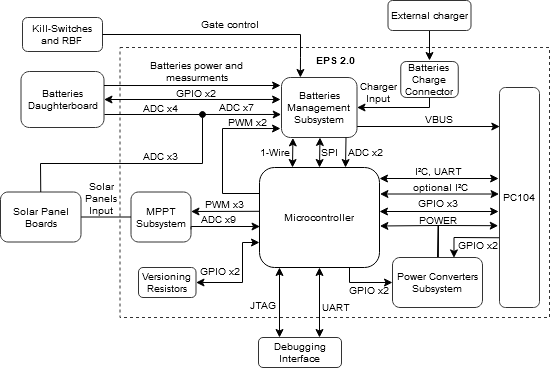
\includegraphics[width=\textwidth]{figures/eps2_mcu_diagram.png}
        \caption{EPS 2.0 MCU Block diagram.}
        \label{fig:mcu-block-diagram}
    \end{center}
\end{figure}

\section{Power Block Diagram}

\begin{figure}[!ht]
    \begin{center}
        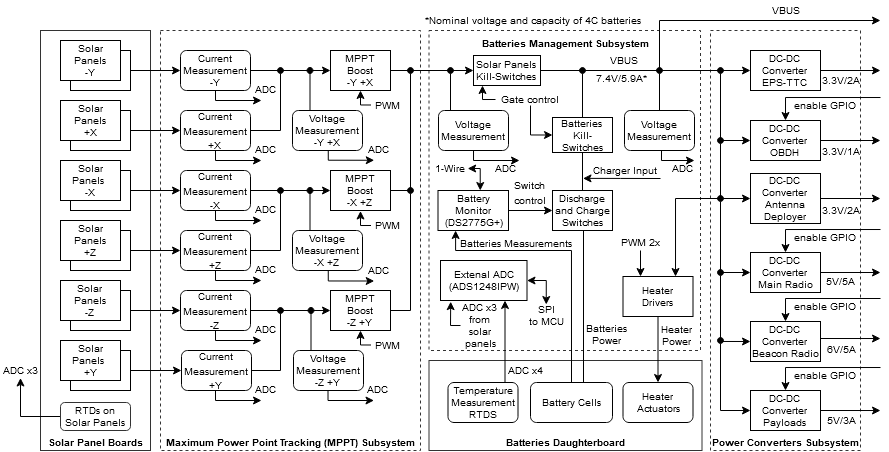
\includegraphics[width=\textwidth]{figures/eps2_power_diagram.png}
        \caption{EPS 2.0 Power Block diagram.}
        \label{fig:power-block-diagram}
    \end{center}
\end{figure}

\section{System Layers} \label{sec:system-layers}



\section{Operation} \label{sec:operation}



\subsection{Execution Flow}



\subsection{Data Flow}



\subsection{Status LEDs} \label{sec:status-leds}